\documentclass[aspectratio=169,10pt]{beamer}

\usepackage[T1]{fontenc}
\usepackage[utf8]{inputenc}
\usepackage[scaled=.96]{helvet}
\renewcommand{\familydefault}{\sfdefault}
\usepackage{booktabs}
\usepackage{array}
\usepackage{listings}
\usepackage{tikz}
\usetikzlibrary{arrows.meta,positioning,shapes.geometric}

% Colours and typography follow the IETF 126 slide deck.
\definecolor{ietfteal}{HTML}{003B49}
\definecolor{ietfblue}{HTML}{176B87}
\definecolor{ietfnavy}{HTML}{003B49}
\definecolor{lightblue}{HTML}{EAF2F4}
\definecolor{softgray}{HTML}{F4F4F4}
\definecolor{darkgray}{HTML}{444444}
\definecolor{pagenumbergray}{HTML}{8C8C8C}
\definecolor{accent}{HTML}{D95F02}
\definecolor{good}{HTML}{2B7A3D}

\setbeamercolor{normal text}{fg=black,bg=white}
\setbeamercolor{structure}{fg=black}
\setbeamercolor{frametitle}{fg=black,bg=white}
\setbeamercolor{title}{fg=white}
\setbeamercolor{subtitle}{fg=lightblue}
\setbeamercolor{author}{fg=white}
\setbeamercolor{date}{fg=lightblue}
\setbeamercolor{block title}{fg=black,bg=softgray}
\setbeamercolor{block body}{fg=black,bg=softgray}
\setbeamercolor{alerted text}{fg=accent}
\setbeamercolor{footline}{fg=pagenumbergray,bg=white}

\setbeamerfont{frametitle}{size=\LARGE,series=\mdseries}
\setbeamerfont{block title}{series=\bfseries}
\setbeamersize{text margin left=.9cm,text margin right=.9cm}

\setbeamertemplate{navigation symbols}{}
\setbeamertemplate{itemize item}{\raise0.1ex\hbox{\small$\bullet$}}
\setbeamertemplate{itemize subitem}{\raise0.1ex\hbox{\scriptsize$\bullet$}}
\setbeamertemplate{footline}{
  \leavevmode%
  \begin{beamercolorbox}[wd=\paperwidth,ht=2.5ex,dp=1.2ex,rightskip=.85cm]{footline}%
    \hfill\insertframenumber
  \end{beamercolorbox}%
}
\setbeamertemplate{frametitle}{
  \nointerlineskip
  \begin{beamercolorbox}[wd=\paperwidth,ht=3.1ex,dp=.85ex,leftskip=.9cm,rightskip=.9cm]{frametitle}
    \usebeamerfont{frametitle}\insertframetitle
  \end{beamercolorbox}
}

\newcommand{\field}[2]{%
  \begin{tikzpicture}[baseline=(n.base)]
    \node[rounded corners=2pt,fill=#1,inner xsep=5pt,inner ysep=2pt,text=white,font=\scriptsize\bfseries] (n) {#2};
  \end{tikzpicture}%
}
\newcommand{\yes}{\textcolor{good}{\bfseries Yes}}
\newcommand{\changed}{\textcolor{accent}{\bfseries Changed}}
\newcommand{\was}[1]{\textcolor{darkgray}{#1}}

\title{Requesting a Freshness Nonce for\\Attestation Evidence in CSRs}
\subtitle{draft-ietf-lamps-attestation-freshness-10}
\author{Hannes Tschofenig, Hendrik Brockhaus, Joe Mandel, Sean Turner}
\date{IETF LAMPS Working Group, IETF 127, November 2026}

\begin{document}

{
\setbeamercolor{background canvas}{bg=white}
\begin{frame}[plain]
  \begin{tikzpicture}[remember picture,overlay]
    \fill[ietfteal]
      (current page.north west) rectangle
      ([yshift=-.80\paperheight]current page.north east);
    \node[anchor=south east,inner sep=0pt]
      at ([xshift=-.72cm,yshift=.23cm]current page.south east)
      {
\includegraphics[width=2.15cm]{ietf-logo.png}};
  \end{tikzpicture}

  \vspace{.28cm}
  {\color{white}\fontsize{24}{27}\selectfont\bfseries\inserttitle\par}
  \vspace{.14cm}
  {\color{white}\fontsize{12}{14}\selectfont\bfseries\insertsubtitle\par}
  \vspace{.55cm}
  {\color{white}\fontsize{10.5}{12}\selectfont\insertauthor\par}
  \vfill
  {\color{white}\fontsize{12}{14}\selectfont\bfseries\insertdate\par}
\end{frame}
}

\begin{frame}{Status since IETF 126}
  \begin{columns}[T,onlytextwidth]
    \begin{column}{0.55\textwidth}
      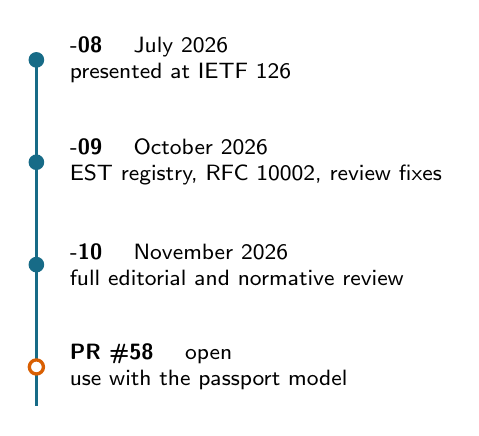
\begin{tikzpicture}[
        x=1cm,y=1cm,
        ev/.style={font=\footnotesize,align=left,anchor=west},
        dot/.style={circle,fill=ietfblue,inner sep=2pt},
        open/.style={circle,draw=accent,very thick,fill=white,inner sep=1.8pt}
      ]
        \draw[very thick,ietfblue] (0,0) -- (0,-4.4);
        \node[dot] at (0,0) {};
        \node[ev] at (.3,0) {\textbf{-08} \quad July 2026\\presented at IETF 126};
        \node[dot] at (0,-1.3) {};
        \node[ev] at (.3,-1.3) {\textbf{-09} \quad October 2026\\EST registry, RFC 10002, review fixes};
        \node[dot] at (0,-2.6) {};
        \node[ev] at (.3,-2.6) {\textbf{-10} \quad November 2026\\full editorial and normative review};
        \node[open] at (0,-3.9) {};
        \node[ev] at (.3,-3.9) {\textbf{PR \#58} \quad open\\use with the passport model};
      \end{tikzpicture}
    \end{column}
    \begin{column}{0.42\textwidth}
      \begin{block}{Two topics today}
        \begin{enumerate}
          \item What changed from -08 to -10
          \item \alert{New:} passport model support (PR \#58)
        \end{enumerate}
      \end{block}
      \vspace{0.2cm}
      \small
      The open issue from IETF 126 (IANA registry for EST path segments) is
      resolved in -09.\\[0.2cm]
      CMC is now a published RFC (RFC 10002), so the normative CMC
      dependency is gone.
    \end{column}
  \end{columns}
\end{frame}

\begin{frame}{Changes from -08 to -10: overview}
  \small
  \begin{columns}[T,onlytextwidth]
    \begin{column}{0.48\textwidth}
      \textbf{\color{ietfblue}Semantics}
      \begin{itemize}
        \item \texttt{expiry} is a hint, not a validity period
        \item \texttt{reqInfo} / \texttt{respInfo} decoupled from \texttt{type} presence
        \item Nonce exchange and CSR \textbf{MUST} share one PKI management
              operation context (was SHOULD)
        \item Lead Attester may pass a derived nonce to sub-Attesters
        \item Non-empty nonce: $\geq$ 64 bits of entropy
      \end{itemize}
    \end{column}
    \begin{column}{0.48\textwidth}
      \textbf{\color{ietfblue}Protocol bindings}
      \begin{itemize}
        \item EST over HTTPS: path segment \texttt{getnonce}
        \item EST: caching disabled, sequential nonce requests only
        \item CMC: Full PKI Request only; references RFC 10002
        \item CMP: registry reference and error handling aligned
      \end{itemize}
      \vspace{0.15cm}
      \textbf{\color{ietfblue}IANA}
      \begin{itemize}
        \item New EST Well-Known URI Path Segments registry
      \end{itemize}
    \end{column}
  \end{columns}
  \vspace{0.1cm}
  \begin{block}{Editorial}
    BCP 14 boilerplate, consistent RATS and PKIX terminology
    (RA/CA, Lead Attester, attestation statement), updated references
    (CSR Attestation -32, RFC 10002, RFC 9111, RFC 8295).
  \end{block}
\end{frame}

\begin{frame}{Message semantics tightened}
  \begin{columns}[T,onlytextwidth]
    \begin{column}{0.48\textwidth}
      \begin{block}{\field{accent}{expiry}\quad now a hint}
        \small
        \begin{itemize}
          \item \was{-08: ``validity period of the nonce''}
          \item -10: how long the RA/CA expects the nonce to remain acceptable;
                a non-negative integer, \texttt{INTEGER (0..MAX)}
          \item The end entity MAY still send Evidence after the period;
                the RA/CA decides whether to accept it
          \item Absent field: no indication given
        \end{itemize}
      \end{block}
    \end{column}
    \begin{column}{0.48\textwidth}
      \begin{block}{\field{ietfblue}{reqTypeInfo}\ \field{ietfblue}{respTypeInfo}}
        \small
        \begin{itemize}
          \item \was{-08: ``if type is set, reqInfo MUST contain \dots''}
          \item -10: \texttt{type} identifies the structure; \texttt{reqInfo}
                and \texttt{respInfo} are simply OPTIONAL
          \item \texttt{len} is the \emph{desired} length; the RA/CA
                SHOULD honour it
        \end{itemize}
      \end{block}
      \vspace{0.15cm}
      \begin{block}{Same transaction, now mandatory}
        \small
        Nonce request/response and the CSR \textbf{MUST} be in the same PKI
        management operation context. The RA/CA treats Evidence as opaque and
        cannot otherwise match a nonce to a CSR.
      \end{block}
    \end{column}
  \end{columns}
\end{frame}

\begin{frame}{EST binding}
  \small
  \begin{tabular}{@{}>{\raggedright\arraybackslash}p{3.4cm}>{\raggedright\arraybackslash}p{4.4cm}>{\raggedright\arraybackslash}p{5.0cm}@{}}
    \toprule
    \textbf{Topic} & \textbf{-08} & \textbf{-10}\\
    \midrule
    HTTPS path segment & \texttt{/nonce} & \texttt{getnonce} (CoAP keeps \texttt{nonce})\\[0.15cm]
    HTTP caching & not addressed & \texttt{Cache-Control: no-store} required\\[0.15cm]
    CoAP caching & not addressed & \texttt{Max-Age} option set to 0\\[0.15cm]
    Several certificates & not addressed & Request the next nonce only after the
      previous CSR has been processed; no interleaved transactions\\[0.15cm]
    Association with CSR & (D)TLS session or cookie & TLS session or cookie (HTTPS);
      DTLS association or Echo option (CoAP)\\
    \bottomrule
  \end{tabular}

  \vspace{0.35cm}
  \begin{block}{Why sequential nonces?}
    EST has no transaction identifier. Session binding can associate one
    outstanding nonce with the next CSR, but not several concurrent ones.
  \end{block}
\end{frame}

\begin{frame}{IANA: EST Well-Known URI Path Segments}
  \begin{columns}[T,onlytextwidth]
    \begin{column}{0.52\textwidth}
      \begin{itemize}
        \item New registry group \textbf{Enrollment over Secure Transport (EST)}
        \item New registry \textbf{EST Well-Known URI Path Segments}
              for segments below \texttt{/.well-known/est}
        \item Columns: Path Segment, Description, Reference
        \item Policy: Specification Required (RFC 8126)
        \item Initial entries collected from RFC 7030, RFC 8295, and RFC 9148
        \item Plus \texttt{getnonce} (HTTP) and \texttt{nonce} (CoAP) from this document
      \end{itemize}
    \end{column}
    \begin{column}{0.44\textwidth}
      \begin{block}{Resolves the IETF 126 open issue}
        EST previously had no registry for path segments, unlike CMP
        (RFC 9811). Merged via PR \#38.
      \end{block}
      \vspace{0.2cm}
      \begin{block}{CMC}
        Simple PKI Request removed: it cannot carry the transaction
        identifier. Only the Full PKI Request is used. ASN.1 module imports
        \texttt{id-mod-enrollMsgSyntax-2025} from RFC 10002.
      \end{block}
    \end{column}
  \end{columns}
\end{frame}

\begin{frame}{PR \#58: why a passport model section?}
  \begin{columns}[T,onlytextwidth]
    \begin{column}{0.55\textwidth}
      \begin{itemize}
        \item The document so far describes only the
              \textbf{background check model}: Evidence in the CSR, RA/CA
              forwards it to a Verifier, RA/CA provides the nonce.
        \item \texttt{draft-ietf-lamps-csr-attestation} explicitly allows an
              \texttt{AttestationStatement} to carry an
              \textbf{Attestation Result} instead of Evidence.
        \item Deployed systems already work this way: the device obtains an
              attestation from a vendor service and presents it to the CA.
        \item Readers asked which model the nonce exchange belongs to.
      \end{itemize}
    \end{column}
    \begin{column}{0.42\textwidth}
      \begin{block}{What the PR adds}
        \begin{itemize}
          \item New Section 7 ``Use with the Passport Model''
          \item Pointer from the architecture section
          \item One paragraph in Security Considerations
          \item Informative references: AR4SI, ACME device attestation
        \end{itemize}
      \end{block}
      \vspace{0.15cm}
      \small No new messages, OIDs, or registrations.
    \end{column}
  \end{columns}
\end{frame}

\begin{frame}{Passport model message flow}
  \centering
  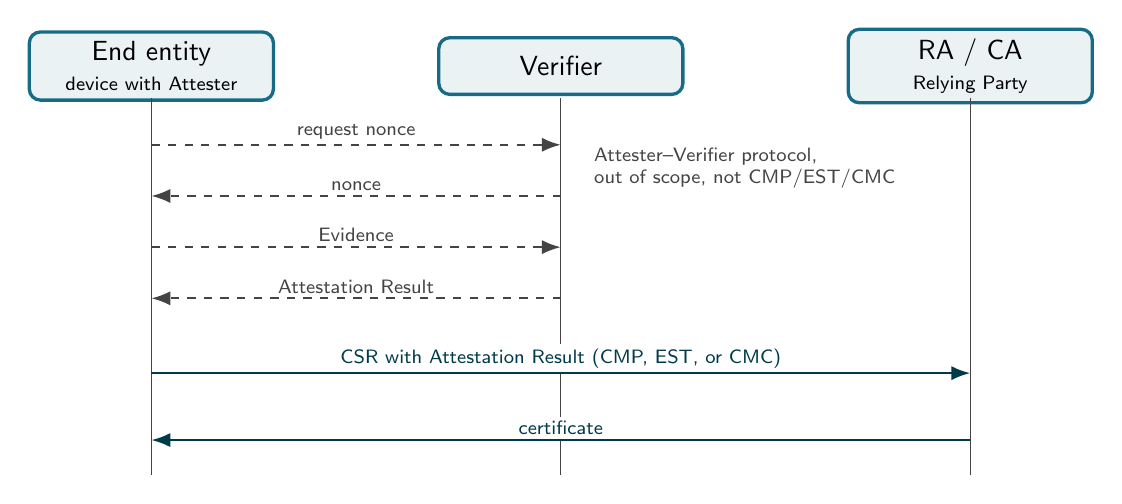
\begin{tikzpicture}[
    x=1cm,y=1cm,
    actor/.style={draw=ietfblue,very thick,rounded corners,fill=lightblue,
                  minimum width=3.1cm,minimum height=.72cm,align=center},
    msg/.style={-{Latex[length=2.4mm]},thick,ietfnavy},
    ext/.style={-{Latex[length=2.4mm]},thick,dashed,darkgray},
    label/.style={font=\scriptsize,fill=white,inner sep=1.5pt}
  ]
    \node[actor] (ee) at (0,0) {End entity\\[-1pt]\scriptsize device with Attester};
    \node[actor] (v)  at (5.2,0) {Verifier};
    \node[actor] (ra) at (10.4,0) {RA / CA\\[-1pt]\scriptsize Relying Party};
    \draw[darkgray] (0,-.4) -- (0,-5.2);
    \draw[darkgray] (5.2,-.4) -- (5.2,-5.2);
    \draw[darkgray] (10.4,-.4) -- (10.4,-5.2);

    \draw[ext] (0,-1.0) -- node[label,above]{request nonce} (5.2,-1.0);
    \draw[ext] (5.2,-1.65) -- node[label,above]{nonce} (0,-1.65);
    \draw[ext] (0,-2.3) -- node[label,above]{Evidence} (5.2,-2.3);
    \draw[ext] (5.2,-2.95) -- node[label,above]{Attestation Result} (0,-2.95);
    \draw[msg] (0,-3.9) -- node[label,above]{CSR with Attestation Result (CMP, EST, or CMC)} (10.4,-3.9);
    \draw[msg] (10.4,-4.75) -- node[label,above]{certificate} (0,-4.75);

    \node[font=\scriptsize,darkgray,align=left,anchor=west] at (5.5,-1.3)
      {Attester--Verifier protocol,\\out of scope, not CMP/EST/CMC};
  \end{tikzpicture}

  \vspace{0.08cm}
  \small
  The Verifier supplies the nonce. The nonce request and response messages of this
  document are \textbf{not used}. The RA/CA receives an Attestation Result, not Evidence.
\end{frame}

\begin{frame}{What the RA/CA checks instead}
  \small
  \begin{columns}[T,onlytextwidth]
    \begin{column}{0.48\textwidth}
      \textbf{Validation of the Attestation Result}
      \begin{itemize}
        \item Produced by a Verifier the RA/CA trusts
        \item Applies to the Attester that generated the key pair
              (binding, see CSR Attestation Section 6.1)
        \item Is fresh
      \end{itemize}
      \vspace{0.15cm}
      \textbf{Freshness without an RA/CA nonce}
      \begin{itemize}
        \item Time information set by the Verifier: issuance time, expiry
        \item Checked against the RA/CA clock and acceptance policy
        \item RFC 9334 Section 10.1 and Appendix A; claims in AR4SI
        \item RA/CA \textbf{SHOULD} define a maximum acceptable age
      \end{itemize}
    \end{column}
    \begin{column}{0.48\textwidth}
      \begin{block}{Replay protection is not freshness}
        Transaction identifiers and nonces of CMP and CMC, or the TLS session
        of EST, protect the enrollment exchange against replay. They say
        nothing about the age of the Attestation Result inside the CSR.
      \end{block}
      \vspace{0.2cm}
      \begin{block}{Security Considerations addition}
        Verifier and RA/CA clocks must be sufficiently synchronized.
        An Attestation Result accepted long after issuance may no longer
        reflect the Attester's state.
      \end{block}
    \end{column}
  \end{columns}
\end{frame}

\begin{frame}{Combining the two models}
  \begin{columns}[T,onlytextwidth]
    \begin{column}{0.50\textwidth}
      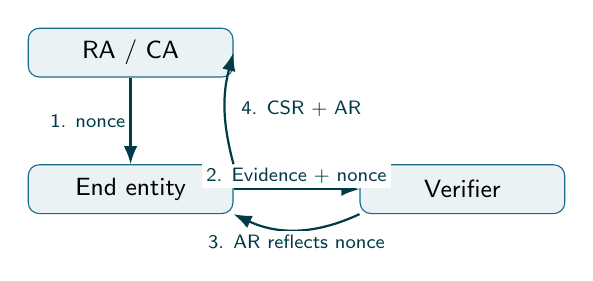
\begin{tikzpicture}[
        node distance=.45cm,
        box/.style={draw=ietfblue,rounded corners,fill=lightblue,
                    minimum width=2.6cm,minimum height=.62cm,align=center,font=\small},
        arr/.style={-{Latex[length=2.3mm]},thick,ietfnavy},
        lbl/.style={font=\scriptsize,fill=white,inner sep=1.5pt}
      ]
        \node[box] (ra) {RA / CA};
        \node[box,below=1.1cm of ra] (ee) {End entity};
        \node[box,right=1.6cm of ee] (v) {Verifier};
        \draw[arr] (ra) -- node[lbl,left]{1. nonce} (ee);
        \draw[arr] (ee.east) -- node[lbl,above]{2. Evidence + nonce} (v.west);
        \draw[arr] (v.south west) to[bend left=25] node[lbl,below]{3. AR reflects nonce} (ee.south east);
        \draw[arr] (ee.north east) to[bend left=15] node[lbl,right,xshift=4pt]{4. CSR + AR} (ra.east);
      \end{tikzpicture}
    \end{column}
    \begin{column}{0.46\textwidth}
      \begin{itemize}
        \item If policy requires a nonce the RA/CA generated itself,
              the nonce exchange of this document can run \emph{before}
              the Attester--Verifier interaction.
        \item The Verifier reflects the nonce into the Attestation Result.
        \item Precedent: \texttt{draft-ietf-acme-device-attest}; the ACME
              challenge token is bound into the vendor-issued attestation.
        \item The PR mentions this pattern but does not specify it.
      \end{itemize}
    \end{column}
  \end{columns}
  \vspace{0.15cm}
  \begin{block}{Question for the WG}
    Keep this as an informative note, or specify the combination in detail?
  \end{block}
\end{frame}

\begin{frame}{The models can be nested}
  \begin{columns}[T,onlytextwidth]
    \begin{column}{0.52\textwidth}
      \small
      \begin{tabular}{@{}p{2.7cm}p{2.0cm}p{2.5cm}@{}}
        \toprule
        & \textbf{Enrollment} & \textbf{Certificate use}\\
        \midrule
        Attester & end entity & end entity\\
        Verifier & Verifier & RA / CA\\
        Relying Party & RA / CA & certificate users\\
        Attestation Result & AR in CSR & the certificate\\
        \bottomrule
      \end{tabular}
      \vspace{0.3cm}

      RFC 9334 Section 5.3 (Figure 7) describes exactly this: Relying Party 2
      hands an Attestation Result back to the Attester for use with Relying
      Party 1.
    \end{column}
    \begin{column}{0.44\textwidth}
      \begin{itemize}
        \item The certificate is issued by a trusted authority after appraisal,
              retained by the Attester, and presented to others.
        \item It does \textbf{not} carry the appraised claims; it attests only
              that the CA's issuance policy was met at issuance time.
        \item Its validity period is independent of the freshness of the
              Evidence.
        \item The nonce mechanism of this document applies to the enrollment
              exchange only.
      \end{itemize}
    \end{column}
  \end{columns}
\end{frame}

\begin{frame}{Summary and next steps}
  \begin{itemize}
    \item -09 and -10 close the IETF 126 open issue and complete a full review
    \item CMC binding now rests on RFC 10002
    \item EST binding has a registry, caching rules, and a clear transaction model
    \item PR \#58 adds informative guidance for the passport model without new
          protocol elements
  \end{itemize}

  \vspace{0.3cm}
  \begin{block}{Asks}
    \begin{enumerate}
      \item Review PR \#58:\\
            \href{https://github.com/lamps-wg/lamps-attestation-freshness/pull/58}{\footnotesize\texttt{https://github.com/lamps-wg/lamps-attestation-freshness/pull/58}}
      \item Should the passport model section stay informative, or do we need
            normative text for the combined flow?
      \item With PR \#58 merged, is the document ready for WGLC?
    \end{enumerate}
  \end{block}
\end{frame}

\end{document}
